\subsection{CLINES architecture and modules}

To leverage the superior performance of large language models within manageable context length, CLINES is designed as a four-step pipeline. Instead of an end-to-end approach--where LLMs often hallucinate or miss instructions in lengthy or complex notes--each key task is modularized and paired with carefully designed prompting strategies. The workflow is illustrated in Figure~\ref{fig:clines-overview}.

\begin{figure}[t!]
  \centering
  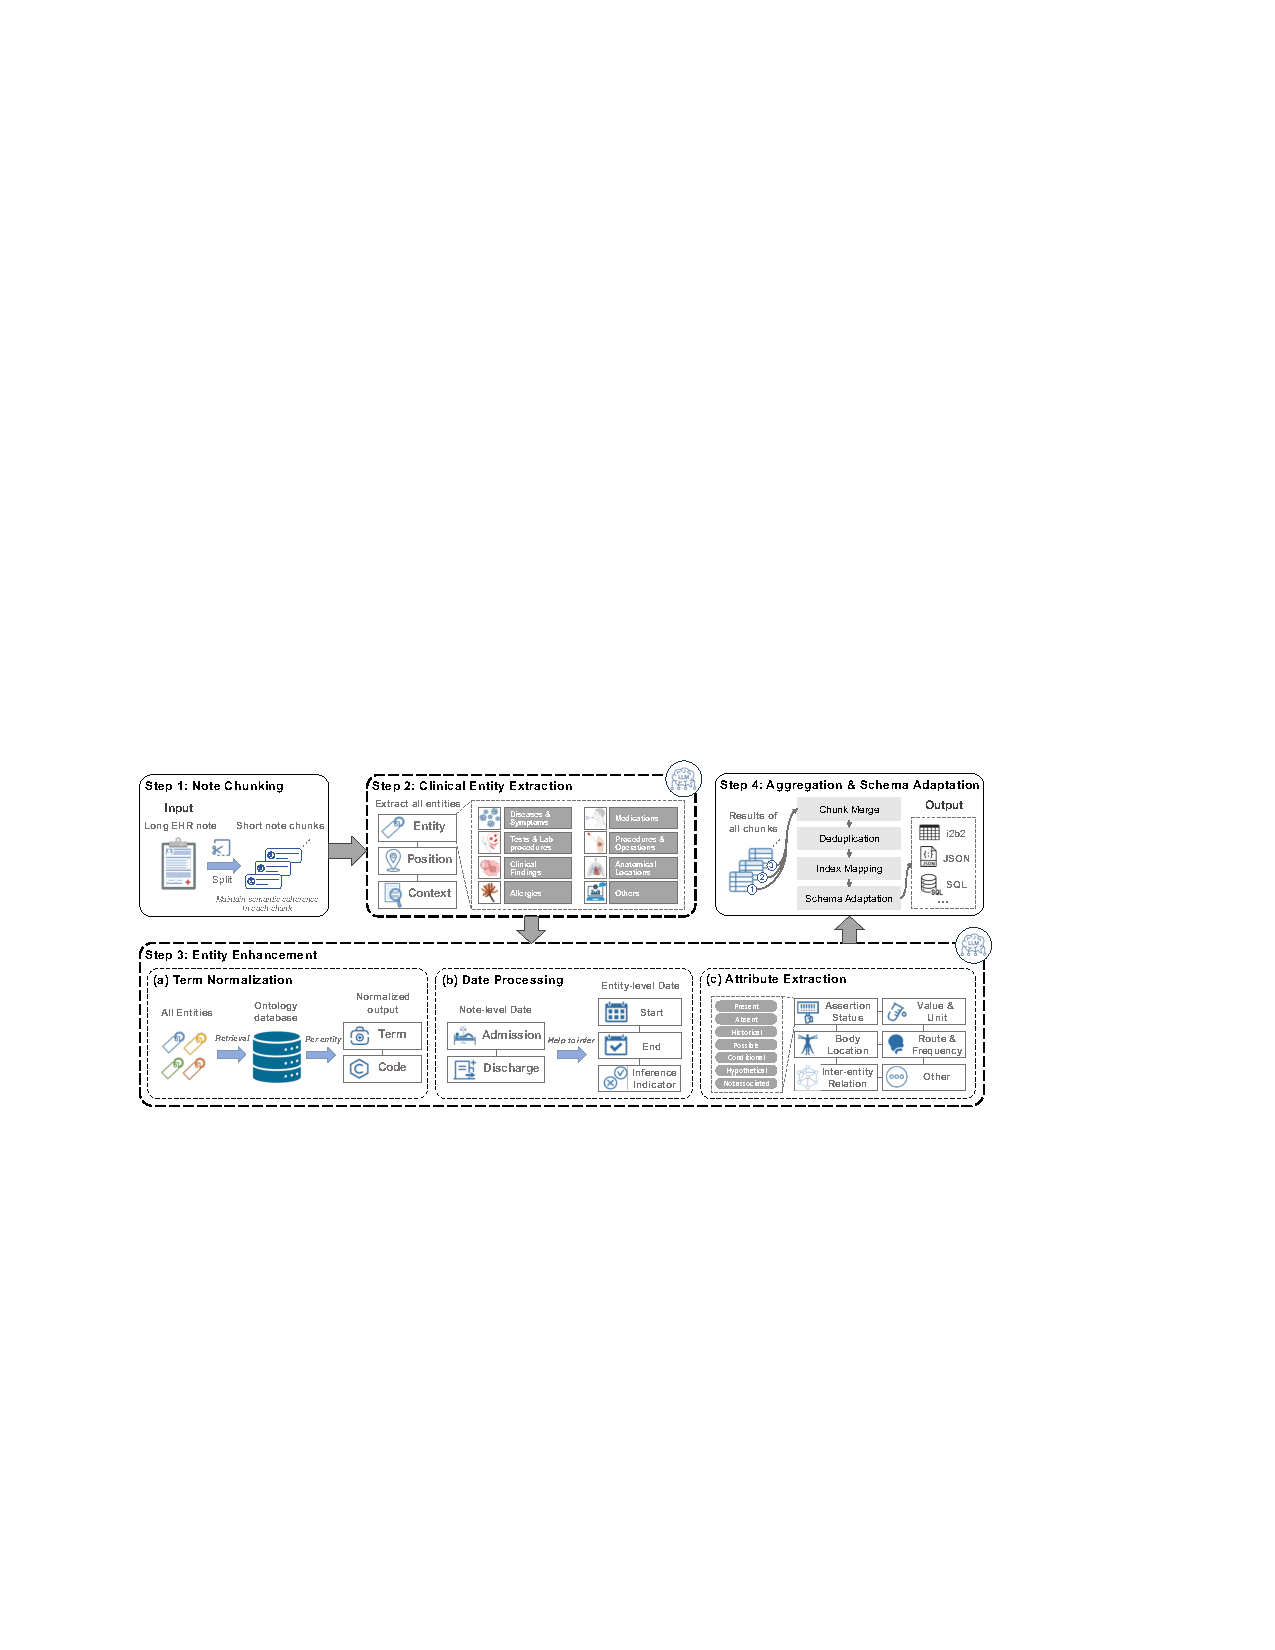
\includegraphics[width=\linewidth,height=0.9\textheight,keepaspectratio]{figures/figure1.pdf}\vspace{-9mm}
  \caption{\textbf{Overview of CLINES.} Step 1, segments long clinical notes into semantically coherent chunks to constrain LLM's context window and improve robustness. Step 2, from each chunk, extract clinical entities with broad coverage, including medications, diseases, and laboratory tests. Step 3, for each entity, uses local context to: (a) normalize to an ontology term with a unique code; (b) for event-type entities, extract or infer start and end dates, when imprecise; and (c) infer assertion status and capture clinically relevant modifiers, e.g., for medications: dose, unit, frequency, and route; for tests: numeric values (with units); for diseases: activity status and other pertinent attributes. Step 4, reconciles entity-level information across all chunks and exports results in user-specified formats (e.g., i2b2, JSON, SQL).}
  \label{fig:clines-overview}
\end{figure}


\paragraph{Step 1 -- Note chunking} Input notes are tokenized with TikToken \cite{tiktoken2024} and segmented using SemChunk \cite{semchunk2024} into semantically coherent fragments of roughly 768 tokens, preserving clinical meaning while fitting LLM context windows. Chunks are processed in parallel to increase throughput. Core metadata (e.g., admission or discharge dates) is retained in all chunks to support temporal alignment. \new{Chunks are non-overlapping (no sliding window is used) and no source text is truncated; the 768-token target is measured after TikToken tokenization. Boundaries fall at sentence and paragraph breaks identified by SemChunk so that a clinical statement is not split mid-sentence, and a single semantic unit larger than the target size is kept intact rather than truncated. SemChunk functions purely as a boundary-detection heuristic and does not by itself guarantee that clinical reasoning spanning multiple chunks is preserved within one chunk; cross-chunk continuity is instead recovered through the metadata replication described here and the Step~4 reconciliation described below, with residual cross-chunk reasoning loss acknowledged as a limitation.}

\paragraph{Step 2 -- Clinical entity extraction} Each chunk is processed to identify relevant mentions (e.g., symptoms, findings, medications) in narrative order, with positions and contexts preserved. Maintaining order captures clinician reasoning flow while isolating core concepts reduces redundancy and simplifies downstream relation, attribute, and temporal extraction.

\paragraph{Step 3 -- Concept and attribute enrichment} \textbf{(a) Term normalization:} Extracted mentions are mapped to ontology concepts (e.g., UMLS) using LLM-assisted disambiguation and SapBERT-based retrieval, where SapBERT \cite{liu2021self} provides biomedical embeddings; candidates are ranked by cosine similarity. \new{The retrieval index type, similarity computation, candidate count, and the UMLS release used to build the concept index are specified in full in Supplementary~\S2.3.} \textbf{(b) Date processing:} Explicit dates are normalized to YYYY-MM-DD. Relative or implicit references (e.g., ``three days post-admission'') are inferred using anchors such as admission and discharge timestamps; ambiguous dates are flagged as inferred. \textbf{(c) Attribute extraction:} For each normalized concept, the pipeline captures assertion status (present, absent, possible, historical), numerical values with inferred units, medication route and frequency, anatomical location, and relations between entities (e.g., infection ``has symptom'' presyncope, ``managed by'' rehydration). This enriched representation supports downstream phenotyping, predictive modeling, and real-world evidence generation \cite{He_2023,Hou_2023}. \new{The relation-extraction component is deployed as part of the structured output but is not benchmarked in this study, because gold-standard relation annotations are unavailable for all four corpora; its quantitative evaluation is deferred to future work (see Limitations).}

\paragraph{Step 4 -- Aggregation and schema adaptation} Outputs are reconciled across chunks through deduplication and cross-segment linking, unifying repeated mentions and preserving longitudinal continuity. \new{Concretely, reconciliation (i) re-indexes chunk-local character offsets to document-global positions and de-duplicates mentions on the (start position, end position, semantic type) key; (ii) resolves conflicting assertion labels for the same mention by the fixed priority present~$>$~historical~$>$~possible~$>$~absent~$>$~not-associated; and (iii) reconciles dates by retaining the most specific non-null resolution unless explicitly contradicted by an earlier chunk. Duplicate mentions arise predominantly from medication brand/generic equivalence and from the same entity recurring across adjacent chunks.} Harmonized outputs are mapped to a standardized schema (e.g., i2b2) or a target schema specified by the use-case, then exported to CSV, JSON, or SQLite for downstream analysis. Module-level dataflow is summarized in Figure~\ref{fig:clines-workflow}.

\begin{figure}[H]
  \centering
  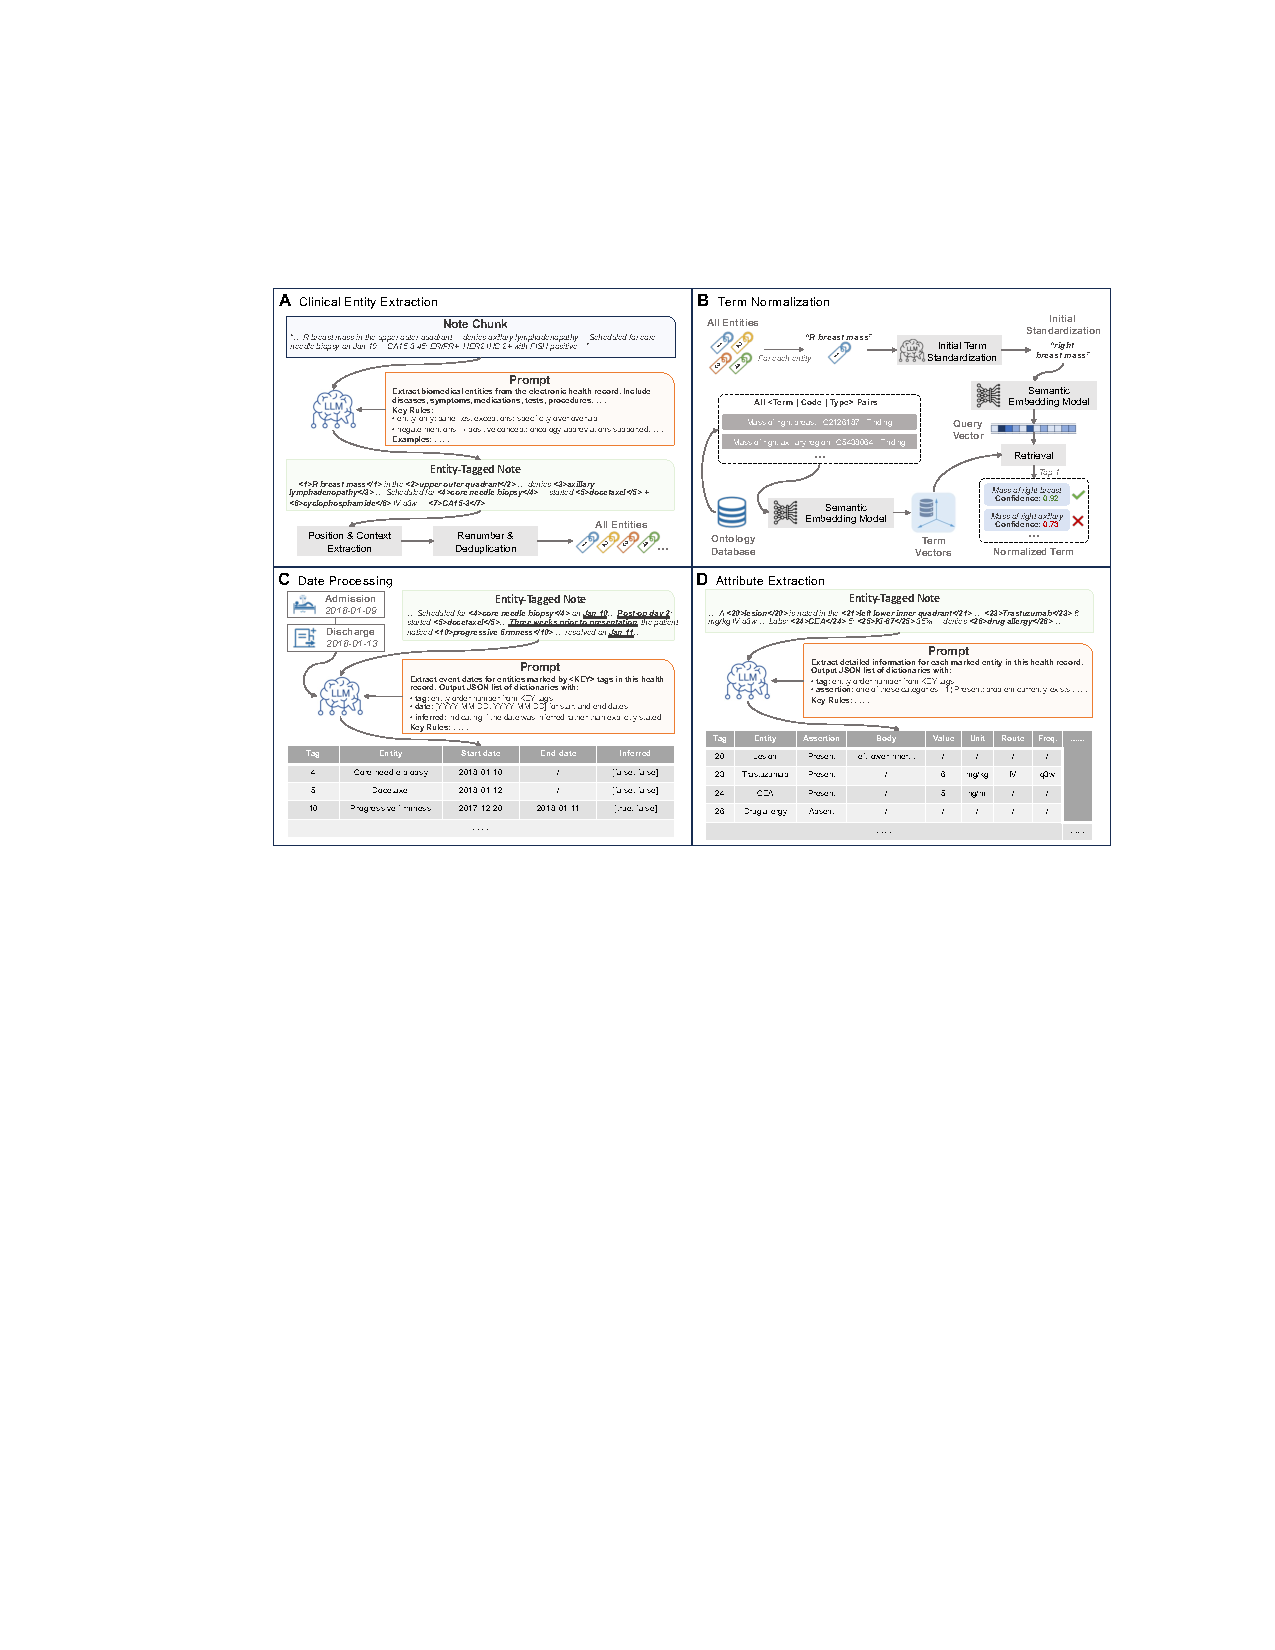
\includegraphics[width=\linewidth,height=0.9\textheight,keepaspectratio]{figures/figure2.pdf}\vspace{-8mm}
  \caption{\textbf{CLINES LLM-based module workflow.} (A) Within each note chunk, the LLM tags clinical entities; post-processing yields an entity list with source offsets and a surrounding context window. (B) The LLM performs preliminary normalization, after which an embedding-based retriever queries the ontology database to return the nearest term, concept code, and semantic type. (C) Explicit dates/times are extracted from local context; when documentation is vague, admission/discharge metadata are used to resolve relative or fuzzy expressions to the most plausible calendar dates. (D) Context is used to capture modifiers (e.g., for medications: dose, unit, frequency, route; for tests: numeric values and units; for diseases: activity status), and to infer latent modifiers implied by panel tests (e.g., default units). All machine-inferred fields are flagged as ``inferred'' to facilitate audit and downstream use.}
  \label{fig:clines-workflow}
\end{figure}


\subsection{Implementation and LLM configuration}

CLINES is model-agnostic; we employed three instruction-finetuned frontier LLMs with identical decoding settings: Llama-3.1-405B (temperature 0.6, max output 8192 tokens; \new{served in FP8 precision---the official \texttt{Meta-Llama-3.1-405B-Instruct-FP8} checkpoint, the lightest weights released by Meta---on 8\(\times\)H100 GPUs via SGLang with eight-way tensor parallelism}), GPT-4o (temperature 0.6, max output 8192), and o3-mini (medium reasoning effort, max output 32768). Notes were chunked to \(\le\)768 tokens of raw text per request. With GPT-4o, mean prompt tokens were \(\approx 8088.25\) and mean completion tokens \(\approx 2795.25\) per chunk; with o3-mini, mean completion tokens increased to \(\approx 24334.50\). GPT-4o and o3-mini were accessed via API (no local GPUs). \new{We distinguish the four \emph{architectural stages} (chunk~$\rightarrow$~extract~$\rightarrow$~enrich~$\rightarrow$~aggregate) from the underlying \emph{LLM invocations}: a single chunk traversal issues several model calls---entity extraction, attribute and assertion classification, date normalization, and JSON-repair helper calls---so the per-note invocation count substantially exceeds four. Exact per-step invocation counts, token usage, wall-clock time, and estimated cost are reported per dataset and model in the cost analysis (Figure~\ref{fig:robustness-cost}b).}

\new{All language-model inference was performed via Harvard Medical School's HIPAA-compliant Azure OpenAI Service tenant, governed by a Business Associate Agreement between Harvard Medical School and Microsoft. Clinical text remained within the HMS-controlled Azure tenant throughout inference; no clinical data were transmitted to or stored by OpenAI directly. Microsoft Azure OpenAI Service does not retain submitted prompts or completions for model training under its service-specific terms, in contrast to the public OpenAI consumer API. This deployment configuration was reviewed for compliance with the data-use agreements of the MIMIC-III, 4CE, and CORAL datasets prior to any inference.}

CLINES outputs were exported to the i2b2 schema, and a read-only web demonstrator populated with results from the credentialed-access CORAL dataset was deployed; access is described in the Data and Code availability section.

\subsection{Study design and data}

All corpora were de-identified and accessed under the respective data-use agreements and governance requirements of each dataset; no patient contact, intervention, or access to identifiable private information occurred. \new{All annotators completed CITI Human Subjects Research training and held the access credentials required for each dataset prior to data access. Because this work analyzes only fully de-identified secondary data that are not readily identifiable, it does not constitute human-subjects research under the U.S. Common Rule (45~CFR~46.104) and did not require Institutional Review Board approval or a formal exemption application at the authors' institution; further detail is provided in the Ethics Approval section.}

\textbf{MIMIC-III} \cite{Johnson_2016}: from 2{,}065{,}096 critical-care notes, 964 notes were sampled and segmented into 2{,}000 paragraphs. Twenty-four paragraphs were manually annotated (one expert per paragraph), yielding 448 clinical phrases: 235 body-location mentions, 128 modifiers (e.g., assertion status), and 144 numerical values with units. Acronym--expansion pairs were treated as single phrases; narrative ``purpose'' attributes were excluded from quantitative analysis.

\textbf{4CE} \cite{Brat_2020}: de-identified notes from patients with a history of COVID-19. Of 56 notes, 21 were annotated, producing 5{,}731 entity mentions with temporal information and attributes; mean document length 1{,}466 words (SD 636).

\textbf{CORAL} \cite{Sushil_2024}: 56 de-identified oncology reports (breast or pancreatic cancer). Twenty-nine notes were annotated and partitioned into two subsets: CORAL--Breast (13 documents, 3{,}900 entity records; mean 1{,}997 words) and CORAL--Pancreas (16 documents, 4{,}717 entity records; mean 1{,}906 words). Across the annotated 4CE + CORAL subsets (14{,}348 entity records), 2{,}517 (17.5\%) contained both a numerical value and a unit, and 5{,}680 (39.6\%) carried explicit temporal information.

\subsection{Annotation protocol}

Five annotators followed a consensus protocol balancing accuracy and efficiency: (i) extract core entity spans while excluding modifiers to avoid redundancy; (ii) infer temporality and assertion status from surrounding context (e.g., ``diagnosed with lung cancer 5 months ago,'' ``rule out pneumonia''); (iii) expand abbreviations and non-standard terms to full medical concepts, later normalized via SapBERT \cite{liu2021self}; (iv) infer missing units for numerical values. Annotation was supported by a custom React-based tool enabling interactive review, conflict resolution, and structured export. All annotators received unified training with shared examples; an independent annotator audited a sample for accuracy and consistency. \new{Throughout, \emph{words} denotes whitespace- and punctuation-delimited tokens (stopwords included; a numeric value together with its unit is counted as a single word), and a \emph{clinical phrase} denotes a contiguous span corresponding to a single UMLS-mappable concept or a single value-plus-unit, as marked by annotators.}

\new{\subsection{Inter-annotator agreement}

To quantify the inherent variability among clinical annotators following the protocol described above, we performed a structured cross-annotation study on three notes per dataset (4CE \(n=3\); CORAL \(n=3\); total 2{,}657 candidate-mention rows). For each note, a second annotator, independent of the original assignment, re-annotated the same AI-suggested draft, blinded to the original annotator's selections.

We report inter-annotator agreement (IAA) using three complementary metrics. The primary metric is the \emph{F1-based IAA} (Dice coefficient), defined as \(2|A \cap B| / (|A| + |B|)\), where \(A\) and \(B\) are the sets of mentions retained by each annotator. F1 is the appropriate primary IAA in span-prediction settings where annotators audit an AI-suggested draft rather than perform blank double-annotation, because the resulting label distribution is highly skewed toward keep (here \(\approx 75\%\) of candidate rows kept by either annotator), conditions under which Cohen's \(\kappa\) suffers from the well-documented two-paradox effect~\cite{Feinstein_1990,Byrt_1993} and systematically underestimates substantive agreement~\cite{Hripcsak_2005}. We additionally report Cohen's \(\kappa\) and the Prevalence- and Bias-Adjusted Kappa (PABAK)~\cite{Byrt_1993} as supplementary measures to address Cohen's paradox.

Annotator review uncovered a small number of recurring structural-disambiguation patterns where guideline ambiguity (rather than substantive clinical disagreement) generated apparent label divergence: (a) AI-suggested mentions whose UMLS semantic type is non-clinical (e.g., Bird, Geographic Area, Calendar Month); (b) candidate spans that match a section header (e.g., \emph{Review of Systems}, \emph{Past Medical History}); (c) header-like attribute types (e.g., Clinical Attribute, Body Location or Region) with \emph{Not associated} or \emph{Absent} assertion status; (d) drug brand/generic duplicates within the same span and value/unit; and (e) standalone severity adjectives (e.g., \emph{moderate}, \emph{severe}). We pre-specified that under the consensus protocol all five patterns should resolve to a uniform DROP decision; the resulting reconciliation is reported alongside raw agreement.

Across the cross-annotated subset, the primary F1-based IAA was \textbf{0.837} (mention-level), with supplementary Cohen's \(\kappa = 0.597\) and PABAK \( = 0.609\); raw agreement was 80.5\%. Under conventions for F1-based IAA in clinical NLP~\cite{Hripcsak_2005}, this represents substantial agreement, consistent with published clinical-NER inter-annotator agreement (e.g., i2b2 2010 challenge \(\kappa = 0.43\)--\(0.60\) for entity-boundary tasks~\cite{Uzuner_2011}). Per-note metrics and the rule-trigger breakdown are reported in Supplementary Table S1. For MIMIC-III, where each paragraph was annotated by a single expert without independent re-annotation, we reframe F1 as agreement-with-annotator rather than as a ground-truth benchmark.}

\subsection{Baselines}

To contextualize performance, we compared classical rule-/lexicon-driven pipelines and compact Transformer encoders, representing the two dominant traditions in clinical NLP.

\textbf{Rule-/lexicon-based systems.} cTAKES \cite{Savova_2010} implements sectioning, sentence boundary detection, tokenization, POS tagging, morphological normalization, UMLS mapping, and ConText for negation, uncertainty, and experiencer; shallow parsing and dependency analysis link entities to attributes. MetaMap \cite{Aronson2001MetaMap} performs POS tagging, variant generation, composite noun-phrase formation, and UMLS matching with heuristic scoring plus statistical word-sense disambiguation; it does not natively extract numerical values, units, or temporal relations.

\textbf{Transformer encoders.} Clinical-MobileBERT and Clinical-DistilBERT \cite{Rohanian_2023,Rohanian_2024} fine-tuned on i2b2-2010 concepts \new{\cite{Uzuner_2011}} were included as parameter-efficient clinical NER baselines. \new{To address the absence of full-size deep-learning comparators, we additionally evaluated two larger, publicly released clinical NER encoders as off-the-shelf baselines (no fine-tuning on our corpora): a BERT-base clinical NER model (\texttt{samrawal/bert-base-uncased\_clinical-ner}, 110M parameters) and a GatorTron-base clinical NER model (345M parameters, derived from the UF/NVIDIA GatorTron encoder~\cite{https://doi.org/10.48550/arxiv.2203.03540}).} Evaluations of these encoders were limited to entity extraction because they do not natively support ontology normalization, attribute extraction, or temporal reasoning. Model configurations and hyperparameters followed the authors' implementations.

\textbf{Single-prompt LLMs.} Llama-3.1-405B and GPT-4o were also evaluated in a single-call setting using a compact prompt specifying the target schema and strict JSON output; notes were chunked only to satisfy context limits, and each chunk was processed once without retrieval, tools, cross-chunk aggregation, or multi-step reasoning.

\subsection{Evaluation metrics and protocol}

In the \new{training-free setting (no task-specific supervised fine-tuning on the annotated test sets; the pipeline relies on prompt engineering with few-shot in-context examples, retrieval-augmented normalization, and post-processing rules, none of which constitute zero-shot learning in the strict sense)}, we evaluated: entity detection (phrase-level precision, recall, F1 with exact-span match); attribute extraction (joint exact match of span and attribute for body location, assertion status, value/unit); date extraction and normalization (agreement with gold ISO dates; relative dates correct if the resolved absolute date matches the gold anchor). For Clinical-MobileBERT/Clinical-DistilBERT we report only NER; for cTAKES and MetaMap we report concept identification and assertion where available. End-to-end structuring, normalization, attribute extraction, and date handling are compared only across systems that produce those outputs. \new{This study is reported in accordance with the MI-CLAIM~\cite{Norgeot_2020} and TRIPOD+AI~\cite{Collins_2024} reporting guidelines for artificial-intelligence studies in healthcare; completed checklists are provided in the supplementary materials, replacing the STROBE checklist of the original submission, which is intended for observational epidemiological studies rather than model development and evaluation.}
